% =====================================================================
%  SUPPLEMENTARY MATERIAL -- submitted as a separate file
%  Every item here is cited from the manuscript.
% =====================================================================
\documentclass[11pt]{article}
\usepackage[margin=1in]{geometry}
\usepackage{booktabs}
\usepackage{graphicx}
\usepackage{amsmath}
\usepackage{tabularx}

\graphicspath{{figures/}}
\renewcommand{\thetable}{S\arabic{table}}
\renewcommand{\thefigure}{S\arabic{figure}}
\newcommand{\cstar}{c^{*}}

\title{Supplementary material for\\
``The escalation tax: measuring what manual model and reasoning-mode
selection costs, and whether a one-shot router recovers it''}
\author{Suseta Datta and Indrajeet Mondal}
\date{}

\begin{document}
\maketitle

This file collects the material referred to from the manuscript: the two validation
gates (Tables~\ref{tab:gate1} and \ref{tab:gate2}), router overhead
(Table~\ref{tab:overhead}), the carbon bracket (Table~\ref{tab:carbon}),
per-family accuracy (Table~\ref{tab:family-accuracy}), the two wider pools in
cost order (Tables~\ref{tab:public-pool} and \ref{tab:hosted-cells}), and six
figures (Figures~\ref{fig:detection} to \ref{fig:hosted-frontier}). Every
number repeats the analysis described in the manuscript and is computed by
the same code.

\begin{table}[ht]
\centering
\caption{Validation gate 1: the two NVML energy sources on the RTX~4060
Laptop GPU (enforced limit 115\,W). Counter values are the mean power implied
by the counter's increase over each window.}
\label{tab:gate1}
\renewcommand{\arraystretch}{1.1}
\begin{tabular}{@{}lrrrl@{}}
\toprule
Source & Idle & Load & Cool-down & Verdict \\
\midrule
Sampled power & 2.4\,W & 75.1\,W & 10.5\,W & Usable \\
Energy counter & 88.3\,W & 127.6\,W & 256.9\,W & Rejected \\
\bottomrule
\end{tabular}
\end{table}

\begin{table}[ht]
\centering
\caption{Validation gate 2: mode separation by model size (60 prompts per
size). Ratio is the median of per-prompt think/no-think token ratios with a
95\% bootstrap interval. Marker ratio is no-think marker density divided by
think-trace marker density.}
\label{tab:gate2}
\renewcommand{\arraystretch}{1.1}
\setlength{\tabcolsep}{5pt}
\begin{tabular}{@{}lccccc@{}}
\toprule
Size & AUC & Tokens (think / no) & Ratio (95\% CI) & Leak & Marker \\
\midrule
0.6B & 0.964 & 1444 / 195 & 13.9 (9.4--19.7) & 0 & 0.040 \\
1.7B & 0.954 & 2053 / 184 & 9.1 (7.6--11.9)  & 0 & 0.034 \\
4B   & 0.928 & 1429 / 149 & 7.0 (5.3--11.5)  & 0 & 0.042 \\
8B   & 0.953 & 1814 / 180 & 9.7 (7.7--17.0)  & 0 & 0.045 \\
\bottomrule
\end{tabular}
\end{table}

\begin{table}[ht]
\centering
\small
\caption{Router overhead per decision, averaged over seeds and both training
objectives. CPU energy is an upper bound, decision time multiplied by
54\,W; GPU energy is metered. The LoRA router is charged the zero-shot
probe's cost. Cascade figures are per verification check, and a query may
need several.}
\label{tab:overhead}
\setlength{\tabcolsep}{4pt}
\begin{tabular}{@{}llrrr@{}}
\toprule
Router & Device & p50 (ms) & p95 (ms) & J/decision \\
\midrule
Direct: TF-IDF + LR & CPU & 0.92 & 1.22 & 0.051 \\
TF-IDF + LR & CPU & 1.70 & 2.18 & 0.096 \\
Features + LightGBM & CPU & 2.90 & 3.18 & 0.157 \\
Features + XGBoost & CPU & 1.89 & 2.14 & 0.102 \\
MiniLM + LR & CPU & 24.13 & 46.64 & 1.432 \\
DeBERTa-v3-small & CPU & 134.75 & 229.14 & 7.555 \\
DistilBERT & CPU & 73.55 & 149.41 & 4.401 \\
Qwen3-0.6B, few-shot & GPU & 43.11 & 62.51 & 2.656 \\
Qwen3-0.6B, LoRA & GPU & 55.76 & 78.53 & 2.924 \\
Qwen3-0.6B, zero-shot & GPU & 55.76 & 78.53 & 2.924 \\
Cascade, per check & GPU & 106.55 & 298.40 & 9.732 \\
\bottomrule
\end{tabular}

\end{table}

\begin{table}[ht]
\centering
\small
\caption{Carbon of the escalation tax under oracle detection, in grams of
CO$_2$e per 1{,}000 queries. Total kWh is the policy's own energy for those
queries and Tax kWh the energy of its tax alone; each carbon figure is Tax
kWh multiplied by the grid intensity beside it. The four intensity columns
are in gCO$_2$e/kWh: 50 for a grid carried by nuclear or hydro, 250 for a
large renewable share, 475 for the figure usually quoted as the global
average, and 700 for a grid carried by coal. They are round values spanning
the range grids occupy, not measurements of a named region.}
\label{tab:carbon}
\begin{tabular}{@{}lrrrrrr@{}}
\toprule
Policy & Total kWh & Tax kWh & 50 & 250 & 475 & 700 \\
\midrule
P1, frugal climb & 0.242 & 0.047 & 2.35 & 11.76 & 22.35 & 32.93 \\
P2, think first & 0.719 & 0.459 & 22.94 & 114.70 & 217.93 & 321.16 \\
P3, sticky high & 0.800 & 0.686 & 34.31 & 171.57 & 325.99 & 480.40 \\
P4, uniform start & 0.438 & 0.254 & 12.71 & 63.55 & 120.74 & 177.94 \\
P4, start skewed to $c_8$ & 0.593 & 0.439 & 21.97 & 109.84 & 208.71 & 307.57 \\
Random, then $c_8$ & 0.585 & 0.432 & 21.60 & 108.01 & 205.22 & 302.43 \\
Oracle & 0.164 & 0.000 & 0.00 & 0.00 & 0.00 & 0.00 \\
\bottomrule
\end{tabular}

\end{table}

\begin{table}[ht]
\centering
\caption{Accuracy of each cell by family, in percent, over 400 prompts per
family.}
\label{tab:family-accuracy}
\begin{tabular}{@{}lrrrr@{}}
\toprule
Cell & All & Math & Code & MCQ \\
\midrule
$c_1$ & 40.2 & 53.0 & 23.2 & 44.2 \\
$c_2$ & 53.0 & 65.2 & 33.8 & 60.0 \\
$c_3$ & 59.5 & 75.2 & 31.0 & 72.2 \\
$c_4$ & 65.0 & 71.0 & 47.2 & 76.8 \\
$c_5$ & 79.0 & 85.5 & 67.5 & 84.0 \\
$c_6$ & 76.8 & 73.0 & 70.0 & 87.2 \\
$c_7$ & 83.6 & 88.2 & 75.2 & 87.2 \\
$c_8$ & 79.8 & 75.2 & 75.0 & 89.0 \\
\bottomrule
\end{tabular}

\end{table}

\begin{table}[ht]
\centering
\footnotesize
\caption{The public pool in cost order, over the 12{,}168 queries of nine
datasets that all thirteen models answered. Cost is the provider's own
charge, in US dollars per 1{,}000 queries. The $\cstar$ share is the fraction
of queries for which that model is the cheapest one that answers correctly,
and the last row the queries no model answers. A bullet marks the four models
on the cost--accuracy frontier, which are the rungs of the escalation ladder.}
\label{tab:public-pool}
\setlength{\tabcolsep}{4pt}
\begin{tabular}{@{}lrrrrc@{}}
\toprule
Model & Acc.\ (\%) & Cost (\$/1{,}000) & \$ per solved (/1{,}000) & $c^*$ share (\%) & Ladder \\
\midrule
\texttt{deepseek-v3-0324} & 41.3 & 0.76 & 1.85 & 7.1 & $\bullet$ \\
\texttt{qwen3-235b-a22b-2507} & 53.3 & 0.84 & 1.58 & 39.4 & $\bullet$ \\
\texttt{deepseek-v3.1-terminus} & 43.5 & 0.99 & 2.27 & 9.6 &  \\
\texttt{kimi-k2-0905} & 44.0 & 1.55 & 3.52 & 4.0 &  \\
\texttt{intern-s1} & 36.9 & 2.81 & 7.61 & 1.9 &  \\
\texttt{gpt-5-chat} & 46.8 & 4.95 & 10.59 & 3.4 &  \\
\texttt{qwen3-235b-a22b-thinking-2507} & 52.1 & 7.52 & 14.43 & 1.5 &  \\
\texttt{gemini-2.5-flash} & 42.7 & 8.63 & 20.23 & 5.7 &  \\
\texttt{claude-sonnet-4} & 37.7 & 10.36 & 27.47 & 0.5 &  \\
\texttt{deepseek-r1-0528} & 47.3 & 13.14 & 27.77 & 1.5 &  \\
\texttt{glm-4.6} & 43.7 & 14.78 & 33.78 & 1.6 &  \\
\texttt{gpt-5} & 57.6 & 29.15 & 50.57 & 3.4 & $\bullet$ \\
\texttt{gemini-2.5-pro} & 58.8 & 60.02 & 102.08 & 2.4 & $\bullet$ \\
\midrule
No model answers & -- & -- & -- & 18.0 &  \\
\bottomrule
\end{tabular}

\end{table}

\begin{table}[ht]
\centering
\footnotesize
\caption{The six hosted cells: three model sizes crossed with two reasoning
efforts, on the prompts of the local main subset. Output tokens include
reasoning tokens, which the provider reports separately but bills as output.
A cap hit is a truncated generation, counted as a failure exactly as a local
cap hit is.}
\label{tab:hosted-cells}
\setlength{\tabcolsep}{3pt}
\begin{tabular}{@{}lllrrrrrrr@{}}
\toprule
Cell & Model & Effort & Cap & Acc.\ (\%) & Acc.\ fin.\ (\%) & Out.\ tok. & Reas.\ tok. & Cap hit (\%) & Cost (\$/1{,}000) \\
\midrule
$h_1$ & \texttt{gpt-5-nano} & Minimal & 2{,}048 & 74.2 & 74.5 & 142 & 0 & 0.5 & 0.03 \\
$h_2$ & \texttt{gpt-5-nano} & High & 4{,}096 & 77.8 & 96.0 & 1{,}908 & 1{,}845 & 18.9 & 0.38 \\
$h_3$ & \texttt{gpt-5-mini} & Minimal & 2{,}048 & 89.5 & 89.6 & 168 & 0 & 0.1 & 0.18 \\
$h_4$ & \texttt{gpt-5-mini} & High & 4{,}096 & 92.8 & 96.5 & 1{,}010 & 886 & 3.8 & 1.02 \\
$h_5$ & \texttt{gpt-5} & Minimal & 2{,}048 & 91.8 & 91.9 & 146 & 0 & 0.1 & 0.79 \\
$h_6$ & \texttt{gpt-5} & High & 4{,}096 & 91.9 & 97.3 & 1{,}140 & 1{,}042 & 5.6 & 5.77 \\
\bottomrule
\end{tabular}

\end{table}

\clearpage

\begin{figure}[ht]
\centering
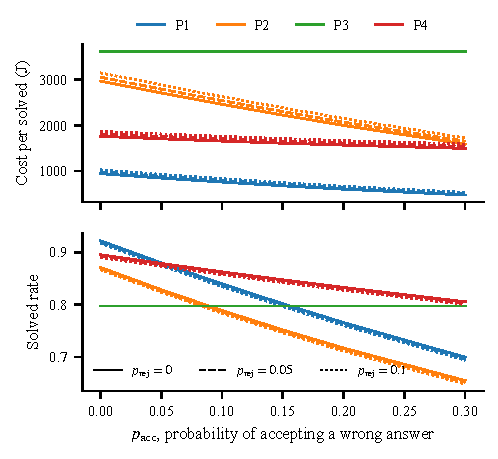
\includegraphics[width=0.8\textwidth]{Figure_S1}
\caption{Cost per solved prompt (top) and solved rate (bottom) of the manual
policies as the probability of accepting a wrong answer grows, at three
probabilities of rejecting a right one. P3 makes a single attempt and keeps
its answer, so detection errors do not move it.}
\label{fig:detection}
\end{figure}

\begin{figure}[ht]
\centering
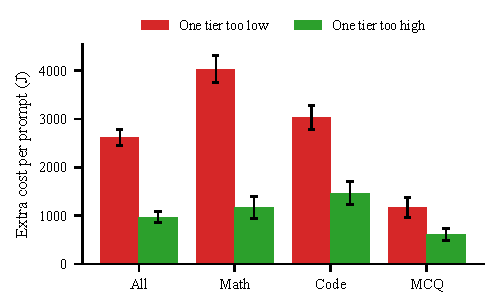
\includegraphics[width=0.8\textwidth]{Figure_S2}
\caption{Extra energy per prompt, over the cost of $\cstar(q)$, of routing
one tier too low and one tier too high, with a failed answer recovered at
$c_8$. Tiers are cells in order of mean energy. Error bars are 95\% bootstrap
intervals.}
\label{fig:asymmetry}
\end{figure}

\begin{figure}[ht]
\centering
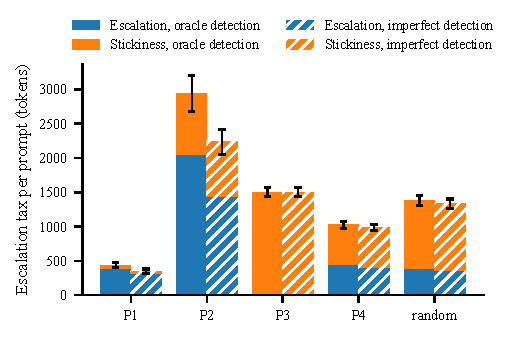
\includegraphics[width=0.8\textwidth]{Figure_S3}
\caption{The escalation tax per prompt counted in tokens, split into
escalation and stickiness, under oracle detection (solid) and imperfect
detection (hatched). Compare Figure~3 of the manuscript, which counts the
same policies in joules and reverses the ranking of P2 and P3.}
\label{fig:tax-tokens}
\end{figure}

\begin{figure}[ht]
\centering
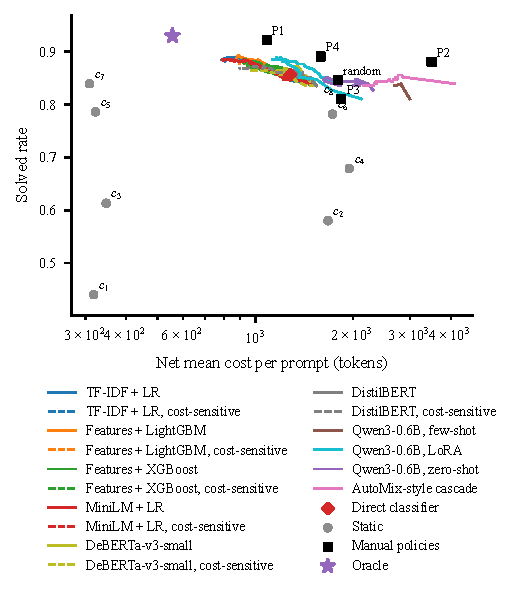
\includegraphics[width=0.8\textwidth]{Figure_S4}
\caption{Solved rate against net mean cost per prompt in tokens on the test
split. Compare Figure~4 of the manuscript, which counts the same routers in
joules; the language-model routers, which pay for their own prompts, fall
behind here.}
\label{fig:frontier-tokens}
\end{figure}

\begin{figure}[ht]
\centering
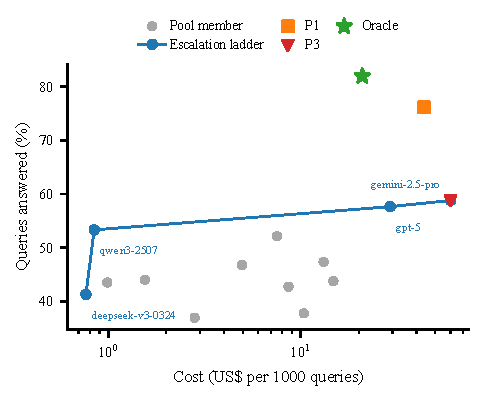
\includegraphics[width=0.8\textwidth]{Figure_S5}
\caption{The thirteen models of the public pool, the cost--accuracy frontier
they define and where the escalation policies land on it. Cost is
logarithmic, in US dollars per 1{,}000 queries. P3 sits on the top rung it
always uses. P1 climbs the frontier and answers more queries than any single
model in the pool, at a price between the two costliest rungs. The oracle
answers still more for a third of what P3 costs.}
\label{fig:public-frontier}
\end{figure}

\begin{figure}[ht]
\centering
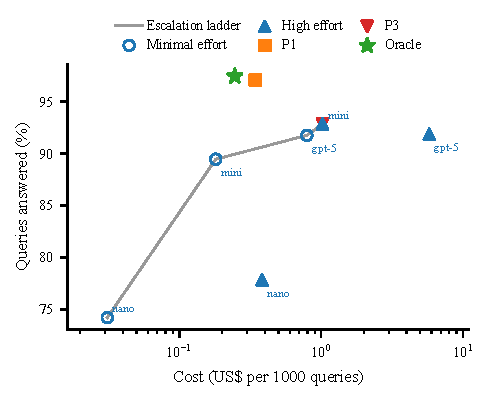
\includegraphics[width=0.8\textwidth]{Figure_S6}
\caption{The six hosted cells on the cost--accuracy plane, open for minimal
reasoning effort and filled for high. Cost is logarithmic, in US dollars per
1{,}000 queries. The grey line is the frontier the escalation policies climb.
The mode axis reads as the horizontal step from an open marker to the filled
marker of the same model.}
\label{fig:hosted-frontier}
\end{figure}

\end{document}
